%%%%%%%%%%%%%%%%%%%%%%%%%%%%%%%%%%%%%%%%%%%%%%%%%%%%%%%%%%%%%%%%%
% Qualificacao de Doutorado / Dept Fisica, CFM, UFSC            %
% Andre@UFSC - 2015                                             %
%%%%%%%%%%%%%%%%%%%%%%%%%%%%%%%%%%%%%%%%%%%%%%%%%%%%%%%%%%%%%%%%%


%:::::::::::::::::::::::::::::::::::::::::::::::::::::::::::::::%
%                                                               %
%                       Anexo: Decomposição                     %
%                                                               %
%:::::::::::::::::::::::::::::::::::::::::::::::::::::::::::::::%

\chapter{Decomposição morfológica espectral e síntese de populações estelares
da amostra final}
\label{apendice:Decomp}


%***************************************************************%
%                                                               %
%                           K0018                               %
%                                                               %
%***************************************************************%

\section{K0018 (NGC 0155)}
\label{apendice:Decomp:K0018}

\begin{itemize}
  \item Galáxia NGC 0155
  \item Tipo morfológico: E1 (mín. E0, máx. S0)
  \item Magnitude absoluta na banda $r$: $-21,85$
  \item Elipticidade: $0,22$
\end{itemize}

\begin{figure}
	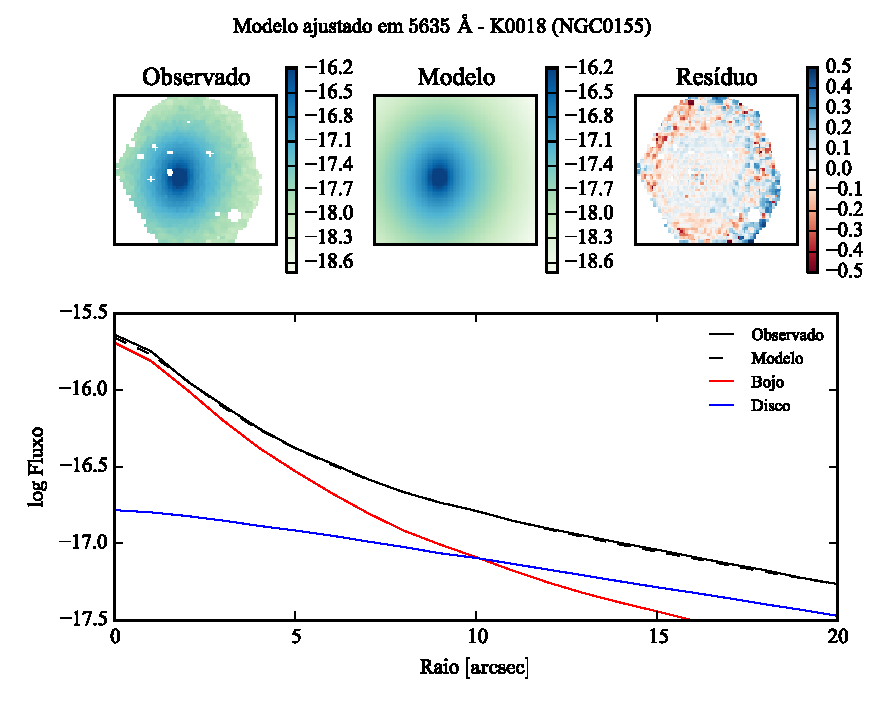
\includegraphics[page=1]{figuras-decomp/K0018_sample006a}
	\caption[Ajuste morfológico em $5635\,\angstrom$ de K0018 (NGC 0155)]
	{Acima: imagens observada, modelada e resíduo, do fluxo em $5635\,\angstrom$
	para K0018 (NGC 0155). Abaixo: perfis radiais, obtidos pela média do fluxo em
	anéis elípticos nas imagens. O fluxo observado é representado pela linha preta
	sólida. O melhor ajuste é representado pela linha preta tracejada. O bojo e o
	disco que compõe o modelo são mostrados em vermelho e azul, respectivamente.}
	\label{fig:decompRadprof:K0018}
\end{figure}

\begin{figure}
	\includegraphics[page=2]{figuras-decomp/K0018_sample006a}
	\caption[Parâmetros morfológicos em função do comprimento de onda de K0018
	(NGC 0155)]
	{Parâmetros morfológicos em função do comprimento de onda para
	K0018 (NGC 0155). Regiões em rosa representam comprimentos de onda onde a
	decomposição falhou. Regiões em cinza foram mascaradas antes de iniciar a
	decomposição. Pontos azuis indicam o primeiro passo da decomposição, em caixas
	de $100\,\angstrom$.}
	\label{fig:decompParams:K0018}
\end{figure}

\begin{figure}
	\includegraphics[page=3]{figuras-decomp/K0018_sample006a}
	\caption[Imagens em $5635\,\angstrom$ das componentes morfológicas de K0018
	(NGC 0155)]
	{Imagens em $5635\,\angstrom$ das componentes morfológicas de K0018
	(NGC 0155).}
	\label{fig:decompImages:K0018}
\end{figure}

\begin{figure}
	\includegraphics[page=4]{figuras-decomp/K0018_sample006a}
	\caption[Espectro das componentes morfológicas de K0018 (NGC 0155)]
	{Espectro das componentes morfológicas de K0018 (NGC 0155),
	observado (preto), bojo (vermelho), disco (azul) e resíduo (magenta). Acima:
	Espectro do {\em spaxel} nuclear da galáxia. Meio: Espectro em um {\em spaxel}
	a uma distância de $r_e$ do núcleo. Abaixo: Espectro integrado espacialmente.}
	\label{fig:decompSpectra:K0018}
\end{figure}

\begin{figure}
	\includegraphics[page=5]{figuras-decomp/K0018_sample006a}
	\caption[Perfis radiais para diversos comprimentos de onda de K0018 (NGC 0155)]
	{Perfis radiais para diversos comprimentos de onda de K0018 (NGC 0155).}
	\label{fig:decompRadprofSpec:K0018}
\end{figure}

\begin{figure}
	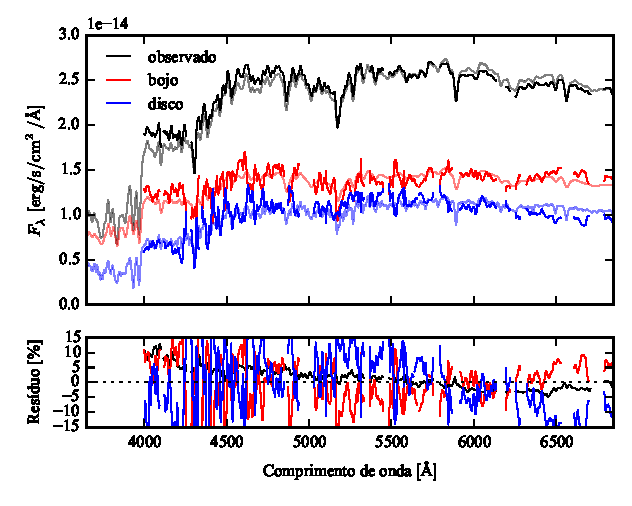
\includegraphics[page=1]{figuras/sample006a_synthesis}
	\caption[Espectros ajustados com \starlight das componentes morfológicas de
	K0018 (NGC 0155)]
	{Acima: Espectros integrados das componentes morfológicas de
	K0018 (NGC 0155), ajustados com \starlight. Em preto, espectro observado. Em
	vermelho, e azul, as componentes bojo e disco. Em linhas de cor clara, o
	espectro ajustado pelo \starlight. Abaixo: Resíduo dos espectros (observado
	menos sintético, divididos pelo observado).}
	\label{fig:decompSintese:K0018}
\end{figure}

\begin{figure}
	\includegraphics[page=2]{figuras/sample006a_synthesis}
	\caption[Propriedades físicas das componentes morfológicas de K0018 (NGC 0155)]
	{Perfil radial de propriedades físicas das componentes morfológicas de
	K0018 (NGC 0155), obtidos através do \starlight. As linhas contínuas
	representam as propriedades obtidas utilizando espectros espacialmente
	resolvidos. As linhas tracejadas representam as propriedades obtidas utilizando
	os espectros integrados. Em preto, espectro observado. Em vermelho, e azul, as
	componentes bojo e disco. Acima, à esquerda: idade estelar média ponderada pela
	luminosidade. Acima, à direita: atenuação por poeira, na banda $V$. Abaixo, à
	esquerda: metalicidade estelar média, ponderada pela massa. Abaixo, à direita:
	densidade superficial de massa estelar. As frações de massa e luminosidade
	entre as componentes e a total (obtida do espectro observado) é mostrada no
	painel inferior, à direita.}
	\label{fig:decompSinteseRadprof:K0018}
\end{figure}

\FloatBarrier

%***************************************************************%
%                                                               %
%                           K0127                               %
%                                                               %
%***************************************************************%

\section{K0127 (NGC 1349)}
\label{apendice:Decomp:K0127}

\begin{itemize}
  \item Galáxia NGC 1349
  \item Tipo morfológico: E6 (mín. E0, máx. Sa)
  \item Magnitude absoluta na banda $r$: $-22,15$
  \item Elipticidade: $0,11$
\end{itemize}

\begin{figure}
	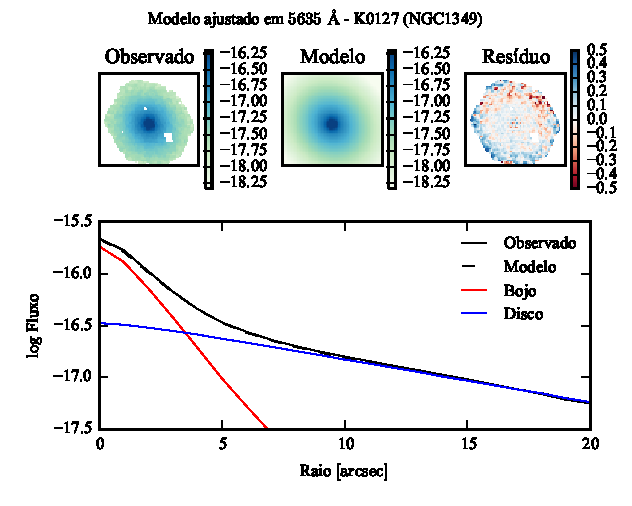
\includegraphics[page=1]{figuras-decomp/K0127_sample006a}
	\caption[Ajuste morfológico em $5635\,\angstrom$ de K0127 (NGC 1349)]
	{Acima: imagens observada, modelada e resíduo, do fluxo em $5635\,\angstrom$
	para K0127 (NGC 1349). Abaixo: perfis radiais, obtidos pela média do fluxo em
	anéis elípticos nas imagens. O fluxo observado é representado pela linha preta
	sólida. O melhor ajuste é representado pela linha preta tracejada. O bojo e o
	disco que compõe o modelo são mostrados em vermelho e azul, respectivamente.}
	\label{fig:decompRadprof:K0127}
\end{figure}

\begin{figure}
	\includegraphics[page=2]{figuras-decomp/K0127_sample006a}
	\caption[Parâmetros morfológicos em função do comprimento de onda de K0127
	(NGC 1349)]
	{Parâmetros morfológicos em função do comprimento de onda para
	K0127 (NGC 1349). Regiões em rosa representam comprimentos de onda onde a
	decomposição falhou. Regiões em cinza foram mascaradas antes de iniciar a
	decomposição. Pontos azuis indicam o primeiro passo da decomposição, em caixas
	de $100\,\angstrom$.}
	\label{fig:decompParams:K0127}
\end{figure}

\begin{figure}
	\includegraphics[page=3]{figuras-decomp/K0127_sample006a}
	\caption[Imagens em $5635\,\angstrom$ das componentes morfológicas de K0127
	(NGC 1349)]
	{Imagens em $5635\,\angstrom$ das componentes morfológicas de K0127
	(NGC 1349).}
	\label{fig:decompImages:K0127}
\end{figure}

\begin{figure}
	\includegraphics[page=4]{figuras-decomp/K0127_sample006a}
	\caption[Espectro das componentes morfológicas de K0127 (NGC 1349)]
	{Espectro das componentes morfológicas de K0127 (NGC 1349),
	observado (preto), bojo (vermelho), disco (azul) e resíduo (magenta). Acima:
	Espectro do {\em spaxel} nuclear da galáxia. Meio: Espectro em um {\em spaxel}
	a uma distância de $r_e$ do núcleo. Abaixo: Espectro integrado espacialmente.}
	\label{fig:decompSpectra:K0127}
\end{figure}

\begin{figure}
	\includegraphics[page=5]{figuras-decomp/K0127_sample006a}
	\caption[Perfis radiais para diversos comprimentos de onda de K0127 (NGC 1349)]
	{Perfis radiais para diversos comprimentos de onda de K0127 (NGC 1349).}
	\label{fig:decompRadprofSpec:K0127}
\end{figure}

\begin{figure}
	\includegraphics[page=3]{figuras/sample006a_synthesis}
	\caption[Espectros ajustados com \starlight das componentes morfológicas de
	K0127 (NGC 1349)]
	{Acima: Espectros integrados das componentes morfológicas de
	K0127 (NGC 1349), ajustados com \starlight. Em preto, espectro observado. Em
	vermelho, e azul, as componentes bojo e disco. Em linhas de cor clara, o
	espectro ajustado pelo \starlight. Abaixo: Resíduo dos espectros (observado
	menos sintético, divididos pelo observado).}
	\label{fig:decompSintese:K0127}
\end{figure}

\begin{figure}
	\includegraphics[page=4]{figuras/sample006a_synthesis}
	\caption[Propriedades físicas das componentes morfológicas de K0127 (NGC 1349)]
	{Perfil radial de propriedades físicas das componentes morfológicas de
	K0127 (NGC 1349), obtidos através do \starlight. As linhas contínuas
	representam as propriedades obtidas utilizando espectros espacialmente
	resolvidos. As linhas tracejadas representam as propriedades obtidas utilizando
	os espectros integrados. Em preto, espectro observado. Em vermelho, e azul, as
	componentes bojo e disco. Acima, à esquerda: idade estelar média ponderada pela
	luminosidade. Acima, à direita: atenuação por poeira, na banda $V$. Abaixo, à
	esquerda: metalicidade estelar média, ponderada pela massa. Abaixo, à direita:
	densidade superficial de massa estelar. As frações de massa e luminosidade
	entre as componentes e a total (obtida do espectro observado) é mostrada no
	painel inferior, à direita.}
	\label{fig:decompSinteseRadprof:K0127}
\end{figure}

\FloatBarrier

%***************************************************************%
%                                                               %
%                           K0592                               %
%                                                               %
%***************************************************************%

\section{K0592 (NGC 4874)}
\label{apendice:Decomp:K0592}

\begin{itemize}
  \item Galáxia NGC 4874
  \item Tipo morfológico: E0 (mín. E0, máx. S0)
  \item Magnitude absoluta na banda $r$: $-22,67$
  \item Elipticidade: $0,12$
\end{itemize}

\begin{figure}
	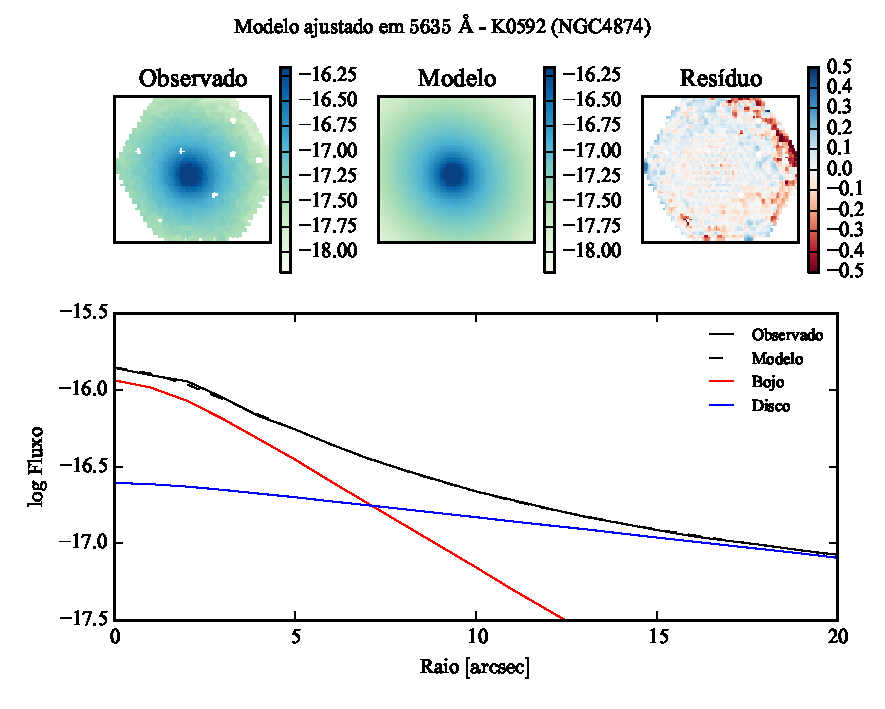
\includegraphics[page=1]{figuras-decomp/K0592_sample006a}
	\caption[Ajuste morfológico em $5635\,\angstrom$ de K0592 (NGC 4874)]
	{Acima: imagens observada, modelada e resíduo, do fluxo em $5635\,\angstrom$
	para K0592 (NGC 4874). Abaixo: perfis radiais, obtidos pela média do fluxo em
	anéis elípticos nas imagens. O fluxo observado é representado pela linha preta
	sólida. O melhor ajuste é representado pela linha preta tracejada. O bojo e o
	disco que compõe o modelo são mostrados em vermelho e azul, respectivamente.}
	\label{fig:decompRadprof:K0592}
\end{figure}

\begin{figure}
	\includegraphics[page=2]{figuras-decomp/K0592_sample006a}
	\caption[Parâmetros morfológicos em função do comprimento de onda de K0592
	(NGC 4874)]
	{Parâmetros morfológicos em função do comprimento de onda para
	K0592 (NGC 4874). Regiões em rosa representam comprimentos de onda onde a
	decomposição falhou. Regiões em cinza foram mascaradas antes de iniciar a
	decomposição. Pontos azuis indicam o primeiro passo da decomposição, em caixas
	de $100\,\angstrom$.}
	\label{fig:decompParams:K0592}
\end{figure}

\begin{figure}
	\includegraphics[page=3]{figuras-decomp/K0592_sample006a}
	\caption[Imagens em $5635\,\angstrom$ das componentes morfológicas de K0592
	(NGC 4874)]
	{Imagens em $5635\,\angstrom$ das componentes morfológicas de K0592
	(NGC 4874).}
	\label{fig:decompImages:K0592}
\end{figure}

\begin{figure}
	\includegraphics[page=4]{figuras-decomp/K0592_sample006a}
	\caption[Espectro das componentes morfológicas de K0592 (NGC 4874)]
	{Espectro das componentes morfológicas de K0592 (NGC 4874),
	observado (preto), bojo (vermelho), disco (azul) e resíduo (magenta). Acima:
	Espectro do {\em spaxel} nuclear da galáxia. Meio: Espectro em um {\em spaxel}
	a uma distância de $r_e$ do núcleo. Abaixo: Espectro integrado espacialmente.}
	\label{fig:decompSpectra:K0592}
\end{figure}

\begin{figure}
	\includegraphics[page=5]{figuras-decomp/K0592_sample006a}
	\caption[Perfis radiais para diversos comprimentos de onda de K0592 (NGC 4874)]
	{Perfis radiais para diversos comprimentos de onda de K0592 (NGC 4874).}
	\label{fig:decompRadprofSpec:K0592}
\end{figure}

\begin{figure}
	\includegraphics[page=5]{figuras/sample006a_synthesis}
	\caption[Espectros ajustados com \starlight das componentes morfológicas de
	K0592 (NGC 4874)]
	{Acima: Espectros integrados das componentes morfológicas de
	K0592 (NGC 4874), ajustados com \starlight. Em preto, espectro observado. Em
	vermelho, e azul, as componentes bojo e disco. Em linhas de cor clara, o
	espectro ajustado pelo \starlight. Abaixo: Resíduo dos espectros (observado
	menos sintético, divididos pelo observado).}
	\label{fig:decompSintese:K0592}
\end{figure}

\begin{figure}
	\includegraphics[page=6]{figuras/sample006a_synthesis}
	\caption[Propriedades físicas das componentes morfológicas de K0592 (NGC 4874)]
	{Perfil radial de propriedades físicas das componentes morfológicas de
	K0592 (NGC 4874), obtidos através do \starlight. As linhas contínuas
	representam as propriedades obtidas utilizando espectros espacialmente
	resolvidos. As linhas tracejadas representam as propriedades obtidas utilizando
	os espectros integrados. Em preto, espectro observado. Em vermelho, e azul, as
	componentes bojo e disco. Acima, à esquerda: idade estelar média ponderada pela
	luminosidade. Acima, à direita: atenuação por poeira, na banda $V$. Abaixo, à
	esquerda: metalicidade estelar média, ponderada pela massa. Abaixo, à direita:
	densidade superficial de massa estelar. As frações de massa e luminosidade
	entre as componentes e a total (obtida do espectro observado) é mostrada no
	painel inferior, à direita.}
	\label{fig:decompSinteseRadprof:K0592}
\end{figure}

\FloatBarrier

%***************************************************************%
%                                                               %
%                           K0602                               %
%                                                               %
%***************************************************************%

\section{K0602 (NGC 4956)}
\label{apendice:Decomp:K0602}

\begin{itemize}
  \item Galáxia NGC 4956
  \item Tipo morfológico: E1 (mín. E0, máx. S0)
  \item Magnitude absoluta na banda $r$: $-21,97$
  \item Elipticidade: $0,14$
\end{itemize}

\begin{figure}
	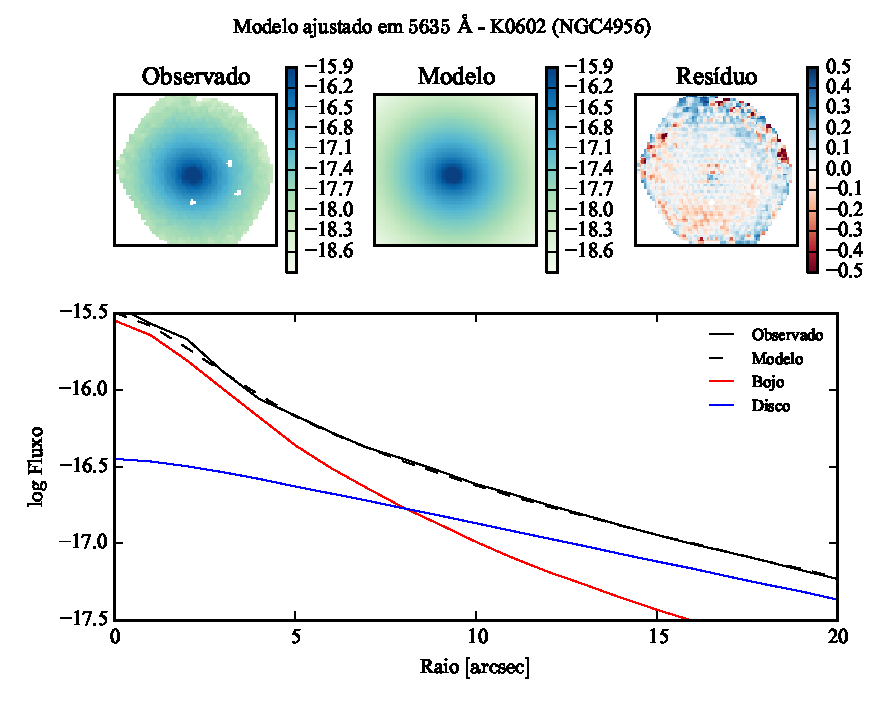
\includegraphics[page=1]{figuras-decomp/K0602_sample006a}
	\caption[Ajuste morfológico em $5635\,\angstrom$ de K0602 (NGC 4956)]
	{Acima: imagens observada, modelada e resíduo, do fluxo em $5635\,\angstrom$
	para K0602 (NGC 4956). Abaixo: perfis radiais, obtidos pela média do fluxo em
	anéis elípticos nas imagens. O fluxo observado é representado pela linha preta
	sólida. O melhor ajuste é representado pela linha preta tracejada. O bojo e o
	disco que compõe o modelo são mostrados em vermelho e azul, respectivamente.}
	\label{fig:decompRadprof:K0602}
\end{figure}

\begin{figure}
	\includegraphics[page=2]{figuras-decomp/K0602_sample006a}
	\caption[Parâmetros morfológicos em função do comprimento de onda de K0602
	(NGC 4956)]
	{Parâmetros morfológicos em função do comprimento de onda para
	K0602 (NGC 4956). Regiões em rosa representam comprimentos de onda onde a
	decomposição falhou. Regiões em cinza foram mascaradas antes de iniciar a
	decomposição. Pontos azuis indicam o primeiro passo da decomposição, em caixas
	de $100\,\angstrom$.}
	\label{fig:decompParams:K0602}
\end{figure}

\begin{figure}
	\includegraphics[page=3]{figuras-decomp/K0602_sample006a}
	\caption[Imagens em $5635\,\angstrom$ das componentes morfológicas de K0602
	(NGC 4956)]
	{Imagens em $5635\,\angstrom$ das componentes morfológicas de K0602
	(NGC 4956).}
	\label{fig:decompImages:K0602}
\end{figure}

\begin{figure}
	\includegraphics[page=4]{figuras-decomp/K0602_sample006a}
	\caption[Espectro das componentes morfológicas de K0602 (NGC 4956)]
	{Espectro das componentes morfológicas de K0602 (NGC 4956),
	observado (preto), bojo (vermelho), disco (azul) e resíduo (magenta). Acima:
	Espectro do {\em spaxel} nuclear da galáxia. Meio: Espectro em um {\em spaxel}
	a uma distância de $r_e$ do núcleo. Abaixo: Espectro integrado espacialmente.}
	\label{fig:decompSpectra:K0602}
\end{figure}

\begin{figure}
	\includegraphics[page=5]{figuras-decomp/K0602_sample006a}
	\caption[Perfis radiais para diversos comprimentos de onda de K0602 (NGC 4956)]
	{Perfis radiais para diversos comprimentos de onda de K0602 (NGC 4956).}
	\label{fig:decompRadprofSpec:K0602}
\end{figure}

\begin{figure}
	\includegraphics[page=7]{figuras/sample006a_synthesis}
	\caption[Espectros ajustados com \starlight das componentes morfológicas de
	K0602 (NGC 4956)]
	{Acima: Espectros integrados das componentes morfológicas de
	K0602 (NGC 4956), ajustados com \starlight. Em preto, espectro observado. Em
	vermelho, e azul, as componentes bojo e disco. Em linhas de cor clara, o
	espectro ajustado pelo \starlight. Abaixo: Resíduo dos espectros (observado
	menos sintético, divididos pelo observado).}
	\label{fig:decompSintese:K0602}
\end{figure}

\begin{figure}
	\includegraphics[page=8]{figuras/sample006a_synthesis}
	\caption[Propriedades físicas das componentes morfológicas de K0602 (NGC 4956)]
	{Perfil radial de propriedades físicas das componentes morfológicas de
	K0602 (NGC 4956), obtidos através do \starlight. As linhas contínuas
	representam as propriedades obtidas utilizando espectros espacialmente
	resolvidos. As linhas tracejadas representam as propriedades obtidas utilizando
	os espectros integrados. Em preto, espectro observado. Em vermelho, e azul, as
	componentes bojo e disco. Acima, à esquerda: idade estelar média ponderada pela
	luminosidade. Acima, à direita: atenuação por poeira, na banda $V$. Abaixo, à
	esquerda: metalicidade estelar média, ponderada pela massa. Abaixo, à direita:
	densidade superficial de massa estelar. As frações de massa e luminosidade
	entre as componentes e a total (obtida do espectro observado) é mostrada no
	painel inferior, à direita.}
	\label{fig:decompSinteseRadprof:K0602}
\end{figure}

\FloatBarrier

%***************************************************************%
%                                                               %
%                           K0832                               %
%                                                               %
%***************************************************************%

\section{K0832 (NGC 6146)}
\label{apendice:Decomp:K0832}

\begin{itemize}
  \item Galáxia NGC 6146
  \item Tipo morfológico: E5 (mín. E3, máx. S0)
  \item Magnitude absoluta na banda $r$: $-22,94$
  \item Elipticidade: $0,23$
\end{itemize}


\begin{figure}
	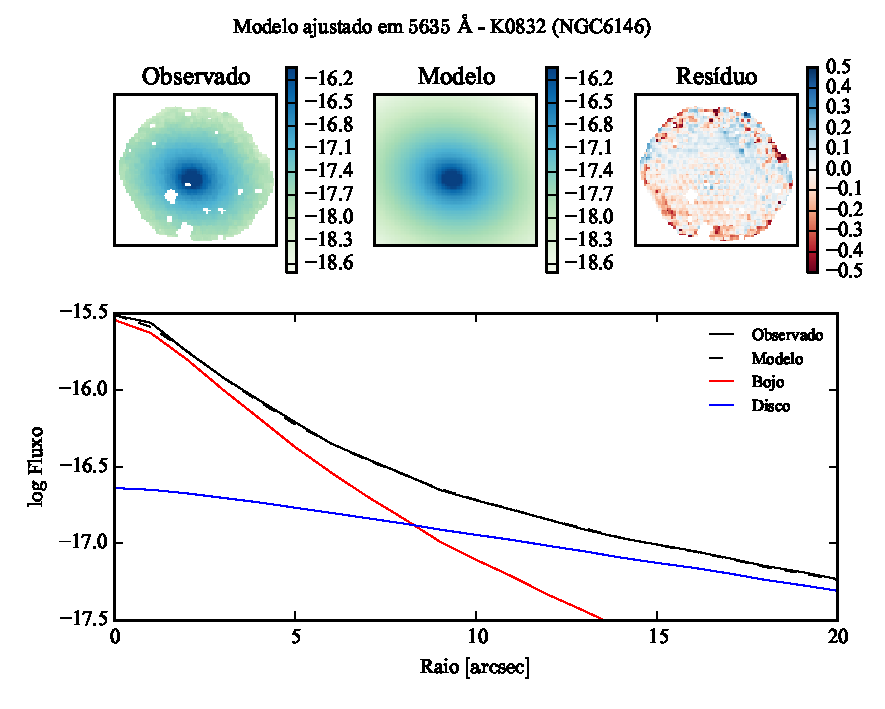
\includegraphics[page=1]{figuras-decomp/K0832_sample006a}
	\caption[Ajuste morfológico em $5635\,\angstrom$ de K0832 (NGC 6146)]
	{Acima: imagens observada, modelada e resíduo, do fluxo em $5635\,\angstrom$
	para K0832 (NGC 6146). Abaixo: perfis radiais, obtidos pela média do fluxo em
	anéis elípticos nas imagens. O fluxo observado é representado pela linha preta
	sólida. O melhor ajuste é representado pela linha preta tracejada. O bojo e o
	disco que compõe o modelo são mostrados em vermelho e azul, respectivamente.}
	\label{fig:decompRadprof:K0832}
\end{figure}

\begin{figure}
	\includegraphics[page=2]{figuras-decomp/K0832_sample006a}
	\caption[Parâmetros morfológicos em função do comprimento de onda de K0832
	(NGC 6146)]
	{Parâmetros morfológicos em função do comprimento de onda para
	K0832 (NGC 6146). Regiões em rosa representam comprimentos de onda onde a
	decomposição falhou. Regiões em cinza foram mascaradas antes de iniciar a
	decomposição. Pontos azuis indicam o primeiro passo da decomposição, em caixas
	de $100\,\angstrom$.}
	\label{fig:decompParams:K0832}
\end{figure}

\begin{figure}
	\includegraphics[page=3]{figuras-decomp/K0832_sample006a}
	\caption[Imagens em $5635\,\angstrom$ das componentes morfológicas de K0832
	(NGC 6146)]
	{Imagens em $5635\,\angstrom$ das componentes morfológicas de K0832
	(NGC 6146).}
	\label{fig:decompImages:K0832}
\end{figure}

\begin{figure}
	\includegraphics[page=4]{figuras-decomp/K0832_sample006a}
	\caption[Espectro das componentes morfológicas de K0832 (NGC 6146)]
	{Espectro das componentes morfológicas de K0832 (NGC 6146),
	observado (preto), bojo (vermelho), disco (azul) e resíduo (magenta). Acima:
	Espectro do {\em spaxel} nuclear da galáxia. Meio: Espectro em um {\em spaxel}
	a uma distância de $r_e$ do núcleo. Abaixo: Espectro integrado espacialmente.}
	\label{fig:decompSpectra:K0832}
\end{figure}

\begin{figure}
	\includegraphics[page=5]{figuras-decomp/K0832_sample006a}
	\caption[Perfis radiais para diversos comprimentos de onda de K0832 (NGC 6146)]
	{Perfis radiais para diversos comprimentos de onda de K0832 (NGC 6146).}
	\label{fig:decompRadprofSpec:K0832}
\end{figure}

\begin{figure}
	\includegraphics[page=9]{figuras/sample006a_synthesis}
	\caption[Espectros ajustados com \starlight das componentes morfológicas de
	K0832 (NGC 6146)]
	{Acima: Espectros integrados das componentes morfológicas de
	K0832 (NGC 6146), ajustados com \starlight. Em preto, espectro observado. Em
	vermelho, e azul, as componentes bojo e disco. Em linhas de cor clara, o
	espectro ajustado pelo \starlight. Abaixo: Resíduo dos espectros (observado
	menos sintético, divididos pelo observado).}
	\label{fig:decompSintese:K0832}
\end{figure}

\begin{figure}
	\includegraphics[page=10]{figuras/sample006a_synthesis}
	\caption[Propriedades físicas das componentes morfológicas de K0832 (NGC 6146)]
	{Perfil radial de propriedades físicas das componentes morfológicas de
	K0832 (NGC 6146), obtidos através do \starlight. As linhas contínuas
	representam as propriedades obtidas utilizando espectros espacialmente
	resolvidos. As linhas tracejadas representam as propriedades obtidas utilizando
	os espectros integrados. Em preto, espectro observado. Em vermelho, e azul, as
	componentes bojo e disco. Acima, à esquerda: idade estelar média ponderada pela
	luminosidade. Acima, à direita: atenuação por poeira, na banda $V$. Abaixo, à
	esquerda: metalicidade estelar média, ponderada pela massa. Abaixo, à direita:
	densidade superficial de massa estelar. As frações de massa e luminosidade
	entre as componentes e a total (obtida do espectro observado) é mostrada no
	painel inferior, à direita.}
	\label{fig:decompSinteseRadprof:K0832}
\end{figure}

\FloatBarrier

%***************************************************************%
%                                                               %
%                           K0846                               %
%                                                               %
%***************************************************************%

\section{K0846 (UGC 10695)}
\label{apendice:Decomp:K0846}

\begin{itemize}
  \item Galáxia UGC 10695
  \item Tipo morfológico: E5 (mín. E2, máx. S0)
  \item Magnitude absoluta na banda $r$: $-22,09$
  \item Elipticidade: $0,33$
\end{itemize}

\begin{figure}
	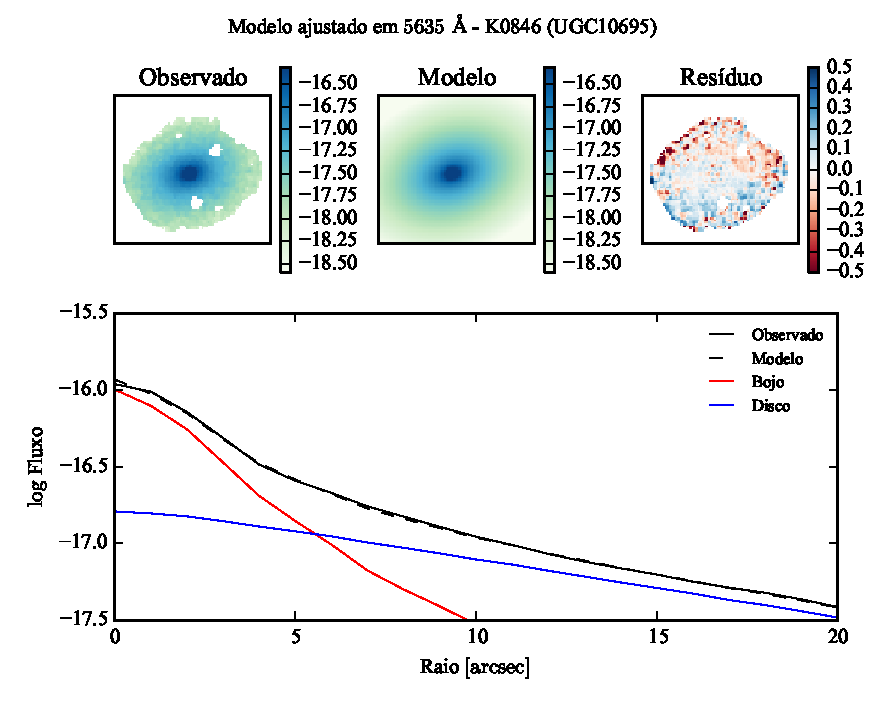
\includegraphics[page=1]{figuras-decomp/K0846_sample006a}
	\caption[Ajuste morfológico em $5635\,\angstrom$ de K0846 (UGC 10695)]
	{Acima: imagens observada, modelada e resíduo, do fluxo em $5635\,\angstrom$
	para K0846 (UGC 10695). Abaixo: perfis radiais, obtidos pela média do fluxo em
	anéis elípticos nas imagens. O fluxo observado é representado pela linha preta
	sólida. O melhor ajuste é representado pela linha preta tracejada. O bojo e o
	disco que compõe o modelo são mostrados em vermelho e azul, respectivamente.}
	\label{fig:decompRadprof:K0846}
\end{figure}

\begin{figure}
	\includegraphics[page=2]{figuras-decomp/K0846_sample006a}
	\caption[Parâmetros morfológicos em função do comprimento de onda de K0846
	(UGC 10695)]
	{Parâmetros morfológicos em função do comprimento de onda para
	K0846 (UGC 10695). Regiões em rosa representam comprimentos de onda onde a
	decomposição falhou. Regiões em cinza foram mascaradas antes de iniciar a
	decomposição. Pontos azuis indicam o primeiro passo da decomposição, em caixas
	de $100\,\angstrom$.}
	\label{fig:decompParams:K0846}
\end{figure}

\begin{figure}
	\includegraphics[page=3]{figuras-decomp/K0846_sample006a}
	\caption[Imagens em $5635\,\angstrom$ das componentes morfológicas de K0846
	(UGC 10695)]
	{Imagens em $5635\,\angstrom$ das componentes morfológicas de K0846
	(UGC 10695).}
	\label{fig:decompImages:K0846}
\end{figure}

\begin{figure}
	\includegraphics[page=4]{figuras-decomp/K0846_sample006a}
	\caption[Espectro das componentes morfológicas de K0846 (UGC 10695)]
	{Espectro das componentes morfológicas de K0846 (UGC 10695),
	observado (preto), bojo (vermelho), disco (azul) e resíduo (magenta). Acima:
	Espectro do {\em spaxel} nuclear da galáxia. Meio: Espectro em um {\em spaxel}
	a uma distância de $r_e$ do núcleo. Abaixo: Espectro integrado espacialmente.}
	\label{fig:decompSpectra:K0846}
\end{figure}

\begin{figure}
	\includegraphics[page=5]{figuras-decomp/K0846_sample006a}
	\caption[Perfis radiais para diversos comprimentos de onda de K0846 (UGC 10695)]
	{Perfis radiais para diversos comprimentos de onda de K0846 (UGC 10695).}
	\label{fig:decompRadprofSpec:K0846}
\end{figure}

\begin{figure}
	\includegraphics[page=11]{figuras/sample006a_synthesis}
	\caption[Espectros ajustados com \starlight das componentes morfológicas de
	K0846 (UGC 10695)]
	{Acima: Espectros integrados das componentes morfológicas de
	K0846 (UGC 10695), ajustados com \starlight. Em preto, espectro observado. Em
	vermelho, e azul, as componentes bojo e disco. Em linhas de cor clara, o
	espectro ajustado pelo \starlight. Abaixo: Resíduo dos espectros (observado
	menos sintético, divididos pelo observado).}
	\label{fig:decompSintese:K0846}
\end{figure}

\begin{figure}
	\includegraphics[page=12]{figuras/sample006a_synthesis}
	\caption[Propriedades físicas das componentes morfológicas de K0846 (UGC 10695)]
	{Perfil radial de propriedades físicas das componentes morfológicas de
	K0846 (UGC 10695), obtidos através do \starlight. As linhas contínuas
	representam as propriedades obtidas utilizando espectros espacialmente
	resolvidos. As linhas tracejadas representam as propriedades obtidas utilizando
	os espectros integrados. Em preto, espectro observado. Em vermelho, e azul, as
	componentes bojo e disco. Acima, à esquerda: idade estelar média ponderada pela
	luminosidade. Acima, à direita: atenuação por poeira, na banda $V$. Abaixo, à
	esquerda: metalicidade estelar média, ponderada pela massa. Abaixo, à direita:
	densidade superficial de massa estelar. As frações de massa e luminosidade
	entre as componentes e a total (obtida do espectro observado) é mostrada no
	painel inferior, à direita.}
	\label{fig:decompSinteseRadprof:K0846}
\end{figure}

\FloatBarrier

%***************************************************************%
%                                                               %
%                           K0851                               %
%                                                               %
%***************************************************************%

\section{K0851 (NGC 6338)}
\label{apendice:Decomp:K0851}

\begin{itemize}
  \item Galáxia NGC 6338
  \item Tipo morfológico: E5 (mín. E1, máx. S0)
  \item Magnitude absoluta na banda $r$: $-22,75$
  \item Elipticidade: $0,34$
\end{itemize}

\begin{figure}
	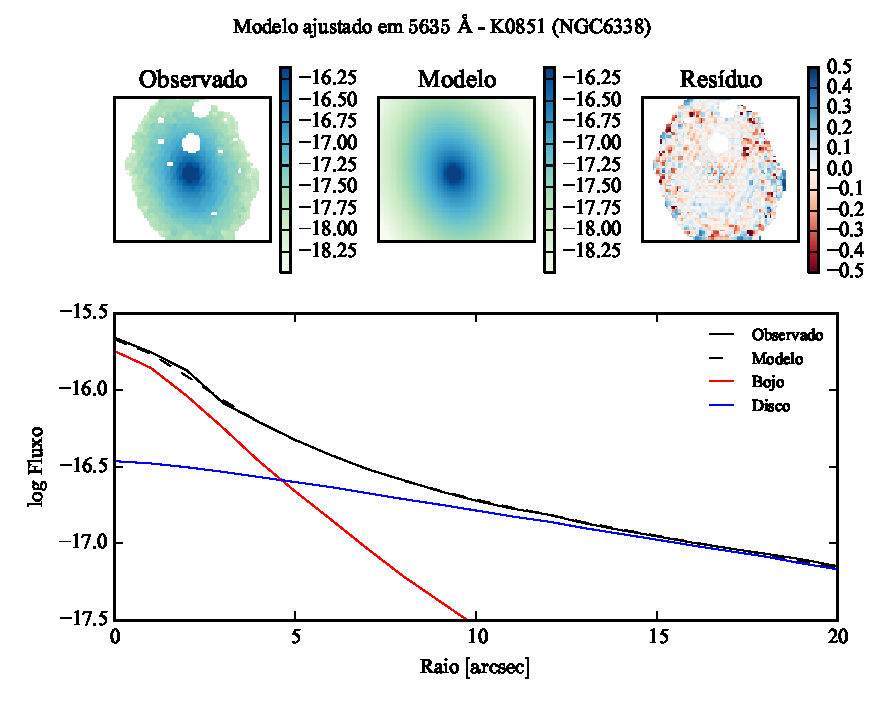
\includegraphics[page=1]{figuras-decomp/K0851_sample006a}
	\caption[Ajuste morfológico em $5635\,\angstrom$ de K0851 (NGC 6338)]
	{Acima: imagens observada, modelada e resíduo, do fluxo em $5635\,\angstrom$
	para K0851 (NGC 6338). Abaixo: perfis radiais, obtidos pela média do fluxo em
	anéis elípticos nas imagens. O fluxo observado é representado pela linha preta
	sólida. O melhor ajuste é representado pela linha preta tracejada. O bojo e o
	disco que compõe o modelo são mostrados em vermelho e azul, respectivamente.}
	\label{fig:decompRadprof:K0851}
\end{figure}

\begin{figure}
	\includegraphics[page=2]{figuras-decomp/K0851_sample006a}
	\caption[Parâmetros morfológicos em função do comprimento de onda de K0851
	(NGC 6338)]
	{Parâmetros morfológicos em função do comprimento de onda para
	K0851 (NGC 6338). Regiões em rosa representam comprimentos de onda onde a
	decomposição falhou. Regiões em cinza foram mascaradas antes de iniciar a
	decomposição. Pontos azuis indicam o primeiro passo da decomposição, em caixas
	de $100\,\angstrom$.}
	\label{fig:decompParams:K0851}
\end{figure}

\begin{figure}
	\includegraphics[page=3]{figuras-decomp/K0851_sample006a}
	\caption[Imagens em $5635\,\angstrom$ das componentes morfológicas de K0851
	(NGC 6338)]
	{Imagens em $5635\,\angstrom$ das componentes morfológicas de K0851
	(NGC 6338).}
	\label{fig:decompImages:K0851}
\end{figure}

\begin{figure}
	\includegraphics[page=4]{figuras-decomp/K0851_sample006a}
	\caption[Espectro das componentes morfológicas de K0851 (NGC 6338)]
	{Espectro das componentes morfológicas de K0851 (NGC 6338),
	observado (preto), bojo (vermelho), disco (azul) e resíduo (magenta). Acima:
	Espectro do {\em spaxel} nuclear da galáxia. Meio: Espectro em um {\em spaxel}
	a uma distância de $r_e$ do núcleo. Abaixo: Espectro integrado espacialmente.}
	\label{fig:decompSpectra:K0851}
\end{figure}

\begin{figure}
	\includegraphics[page=5]{figuras-decomp/K0851_sample006a}
	\caption[Perfis radiais para diversos comprimentos de onda de K0851 (NGC 6338)]
	{Perfis radiais para diversos comprimentos de onda de K0851 (NGC 6338).}
	\label{fig:decompRadprofSpec:K0851}
\end{figure}

\begin{figure}
	\includegraphics[page=13]{figuras/sample006a_synthesis}
	\caption[Espectros ajustados com \starlight das componentes morfológicas de
	K0851 (NGC 6338)]
	{Acima: Espectros integrados das componentes morfológicas de
	K0851 (NGC 6338), ajustados com \starlight. Em preto, espectro observado. Em
	vermelho, e azul, as componentes bojo e disco. Em linhas de cor clara, o
	espectro ajustado pelo \starlight. Abaixo: Resíduo dos espectros (observado
	menos sintético, divididos pelo observado).}
	\label{fig:decompSintese:K0851}
\end{figure}

\begin{figure}
	\includegraphics[page=14]{figuras/sample006a_synthesis}
	\caption[Propriedades físicas das componentes morfológicas de K0851 (NGC 6338)]
	{Perfil radial de propriedades físicas das componentes morfológicas de
	K0851 (NGC 6338), obtidos através do \starlight. As linhas contínuas
	representam as propriedades obtidas utilizando espectros espacialmente
	resolvidos. As linhas tracejadas representam as propriedades obtidas utilizando
	os espectros integrados. Em preto, espectro observado. Em vermelho, e azul, as
	componentes bojo e disco. Acima, à esquerda: idade estelar média ponderada pela
	luminosidade. Acima, à direita: atenuação por poeira, na banda $V$. Abaixo, à
	esquerda: metalicidade estelar média, ponderada pela massa. Abaixo, à direita:
	densidade superficial de massa estelar. As frações de massa e luminosidade
	entre as componentes e a total (obtida do espectro observado) é mostrada no
	painel inferior, à direita.}
	\label{fig:decompSinteseRadprof:K0851}
\end{figure}

\FloatBarrier

%***************************************************************%
%                                                               %
%                           K0858                               %
%                                                               %
%***************************************************************%

\section{K0858 (UGC 10905)}
\label{apendice:Decomp:K00858}

\begin{itemize}
  \item Galáxia UGC 10905
  \item Tipo morfológico: S0a (mín. E7, máx. Sab)
  \item Magnitude absoluta na banda $r$: $-22,32$
  \item Elipticidade: $0,47$
\end{itemize}

\begin{figure}
	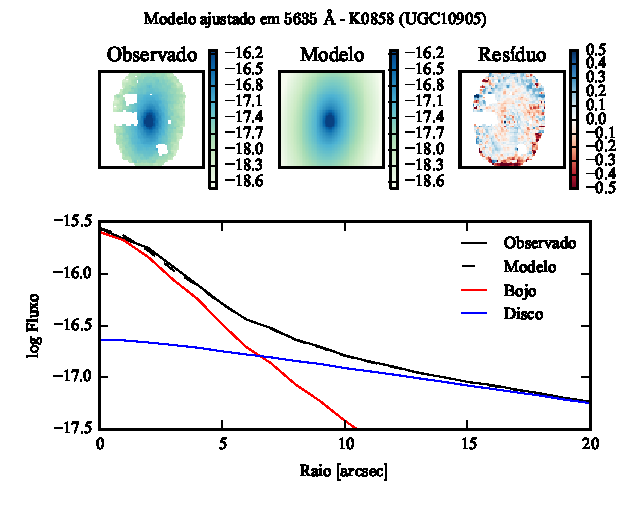
\includegraphics[page=1]{figuras-decomp/K0858_sample006a}
	\caption[Ajuste morfológico em $5635\,\angstrom$ de K0858 (UGC 10905)]
	{Acima: imagens observada, modelada e resíduo, do fluxo em $5635\,\angstrom$
	para K0858 (UGC 10905). Abaixo: perfis radiais, obtidos pela média do fluxo em
	anéis elípticos nas imagens. O fluxo observado é representado pela linha preta
	sólida. O melhor ajuste é representado pela linha preta tracejada. O bojo e o
	disco que compõe o modelo são mostrados em vermelho e azul, respectivamente.}
	\label{fig:decompRadprof:K0858}
\end{figure}

\begin{figure}
	\includegraphics[page=2]{figuras-decomp/K0858_sample006a}
	\caption[Parâmetros morfológicos em função do comprimento de onda de K0858
	(UGC 10905)]
	{Parâmetros morfológicos em função do comprimento de onda para
	K0858 (UGC 10905). Regiões em rosa representam comprimentos de onda onde a
	decomposição falhou. Regiões em cinza foram mascaradas antes de iniciar a
	decomposição. Pontos azuis indicam o primeiro passo da decomposição, em caixas
	de $100\,\angstrom$.}
	\label{fig:decompParams:K0858}
\end{figure}

\begin{figure}
	\includegraphics[page=3]{figuras-decomp/K0858_sample006a}
	\caption[Imagens em $5635\,\angstrom$ das componentes morfológicas de K0858
	(UGC 10905)]
	{Imagens em $5635\,\angstrom$ das componentes morfológicas de K0858
	(UGC 10905).}
	\label{fig:decompImages:K0858}
\end{figure}

\begin{figure}
	\includegraphics[page=4]{figuras-decomp/K0858_sample006a}
	\caption[Espectro das componentes morfológicas de K0858 (UGC 10905)]
	{Espectro das componentes morfológicas de K0858 (UGC 10905),
	observado (preto), bojo (vermelho), disco (azul) e resíduo (magenta). Acima:
	Espectro do {\em spaxel} nuclear da galáxia. Meio: Espectro em um {\em spaxel}
	a uma distância de $r_e$ do núcleo. Abaixo: Espectro integrado espacialmente.}
	\label{fig:decompSpectra:K0858}
\end{figure}

\begin{figure}
	\includegraphics[page=5]{figuras-decomp/K0858_sample006a}
	\caption[Perfis radiais para diversos comprimentos de onda de K0858 (UGC 10905)]
	{Perfis radiais para diversos comprimentos de onda de K0858 (UGC 10905).}
	\label{fig:decompRadprofSpec:K0858}
\end{figure}

\begin{figure}
	\includegraphics[page=15]{figuras/sample006a_synthesis}
	\caption[Espectros ajustados com \starlight das componentes morfológicas de
	K0858 (UGC 10905)]
	{Acima: Espectros integrados das componentes morfológicas de
	K0858 (UGC 10905), ajustados com \starlight. Em preto, espectro observado. Em
	vermelho, e azul, as componentes bojo e disco. Em linhas de cor clara, o
	espectro ajustado pelo \starlight. Abaixo: Resíduo dos espectros (observado
	menos sintético, divididos pelo observado).}
	\label{fig:decompSintese:K0858}
\end{figure}

\begin{figure}
	\includegraphics[page=16]{figuras/sample006a_synthesis}
	\caption[Propriedades físicas das componentes morfológicas de K0858 (UGC 10905)]
	{Perfil radial de propriedades físicas das componentes morfológicas de
	K0858 (UGC 10905), obtidos através do \starlight. As linhas contínuas
	representam as propriedades obtidas utilizando espectros espacialmente
	resolvidos. As linhas tracejadas representam as propriedades obtidas utilizando
	os espectros integrados. Em preto, espectro observado. Em vermelho, e azul, as
	componentes bojo e disco. Acima, à esquerda: idade estelar média ponderada pela
	luminosidade. Acima, à direita: atenuação por poeira, na banda $V$. Abaixo, à
	esquerda: metalicidade estelar média, ponderada pela massa. Abaixo, à direita:
	densidade superficial de massa estelar. As frações de massa e luminosidade
	entre as componentes e a total (obtida do espectro observado) é mostrada no
	painel inferior, à direita.}
	\label{fig:decompSinteseRadprof:K0858}
\end{figure}

\FloatBarrier

%***************************************************************%
%                                                               %
%                           K0912                               %
%                                                               %
%***************************************************************%

\section{K0912 (NGC 7623)}
\label{apendice:Decomp:K0912}

\begin{itemize}
  \item Galáxia NGC 7623
  \item Tipo morfológico: S0 (mín. S0, máx. S0)
  \item Magnitude absoluta na banda $r$: $-21,97$
  \item Elipticidade: $0,14$
\end{itemize}

\begin{figure}
	\includegraphics[page=1]{figuras-decomp/K0912_sample006a}
	\caption[Ajuste morfológico em $5635\,\angstrom$ de K0912 (NGC 7623)]
	{Acima: imagens observada, modelada e resíduo, do fluxo em $5635\,\angstrom$
	para K0912 (NGC 7623). Abaixo: perfis radiais, obtidos pela média do fluxo em
	anéis elípticos nas imagens. O fluxo observado é representado pela linha preta
	sólida. O melhor ajuste é representado pela linha preta tracejada. O bojo e o
	disco que compõe o modelo são mostrados em vermelho e azul, respectivamente.}
	\label{fig:decompRadprof:K0912}
\end{figure}

\begin{figure}
	\includegraphics[page=2]{figuras-decomp/K0912_sample006a}
	\caption[Parâmetros morfológicos em função do comprimento de onda de K0912
	(NGC 7623)]
	{Parâmetros morfológicos em função do comprimento de onda para
	K0912 (NGC 7623). Regiões em rosa representam comprimentos de onda onde a
	decomposição falhou. Regiões em cinza foram mascaradas antes de iniciar a
	decomposição. Pontos azuis indicam o primeiro passo da decomposição, em caixas
	de $100\,\angstrom$.}
	\label{fig:decompParams:K0912}
\end{figure}

\begin{figure}
	\includegraphics[page=3]{figuras-decomp/K0912_sample006a}
	\caption[Imagens em $5635\,\angstrom$ das componentes morfológicas de K0912
	(NGC 7623)]
	{Imagens em $5635\,\angstrom$ das componentes morfológicas de K0912
	(NGC 7623).}
	\label{fig:decompImages:K0912}
\end{figure}

\begin{figure}
	\includegraphics[page=4]{figuras-decomp/K0912_sample006a}
	\caption[Espectro das componentes morfológicas de K0912 (NGC 7623)]
	{Espectro das componentes morfológicas de K0912 (NGC 7623),
	observado (preto), bojo (vermelho), disco (azul) e resíduo (magenta). Acima:
	Espectro do {\em spaxel} nuclear da galáxia. Meio: Espectro em um {\em spaxel}
	a uma distância de $r_e$ do núcleo. Abaixo: Espectro integrado espacialmente.}
	\label{fig:decompSpectra:K0912}
\end{figure}

\begin{figure}
	\includegraphics[page=5]{figuras-decomp/K0912_sample006a}
	\caption[Perfis radiais para diversos comprimentos de onda de K0912 (NGC 7623)]
	{Perfis radiais para diversos comprimentos de onda de K0912 (NGC 7623).}
	\label{fig:decompRadprofSpec:K0912}
\end{figure}

\begin{figure}
	\includegraphics[page=17]{figuras/sample006a_synthesis}
	\caption[Espectros ajustados com \starlight das componentes morfológicas de
	K0912 (NGC 7623)]
	{Acima: Espectros integrados das componentes morfológicas de
	K0912 (NGC 7623), ajustados com \starlight. Em preto, espectro observado. Em
	vermelho, e azul, as componentes bojo e disco. Em linhas de cor clara, o
	espectro ajustado pelo \starlight. Abaixo: Resíduo dos espectros (observado
	menos sintético, divididos pelo observado).}
	\label{fig:decompSintese:K0912}
\end{figure}

\begin{figure}
	\includegraphics[page=18]{figuras/sample006a_synthesis}
	\caption[Propriedades físicas das componentes morfológicas de K0912 (NGC 7623)]
	{Perfil radial de propriedades físicas das componentes morfológicas de
	K0912 (NGC 7623), obtidos através do \starlight. As linhas contínuas
	representam as propriedades obtidas utilizando espectros espacialmente
	resolvidos. As linhas tracejadas representam as propriedades obtidas utilizando
	os espectros integrados. Em preto, espectro observado. Em vermelho, e azul, as
	componentes bojo e disco. Acima, à esquerda: idade estelar média ponderada pela
	luminosidade. Acima, à direita: atenuação por poeira, na banda $V$. Abaixo, à
	esquerda: metalicidade estelar média, ponderada pela massa. Abaixo, à direita:
	densidade superficial de massa estelar. As frações de massa e luminosidade
	entre as componentes e a total (obtida do espectro observado) é mostrada no
	painel inferior, à direita.}
	\label{fig:decompSinteseRadprof:K0912}
\end{figure}

% End of this chapter
